\documentclass[tikz,border=2,dvspsnames]{standalone}
\usetikzlibrary{shadows,arrows,arrows.meta,shapes,positioning,calc,backgrounds,fit}
\newcommand{\vanish}[1]{}
% Define the layers to draw the diagram
%
\definecolor{s1}{HTML}{F1BB7B}
\definecolor{s2}{HTML}{FD6467}
\definecolor{s3}{HTML}{5B1A18}
\begin{document}
%
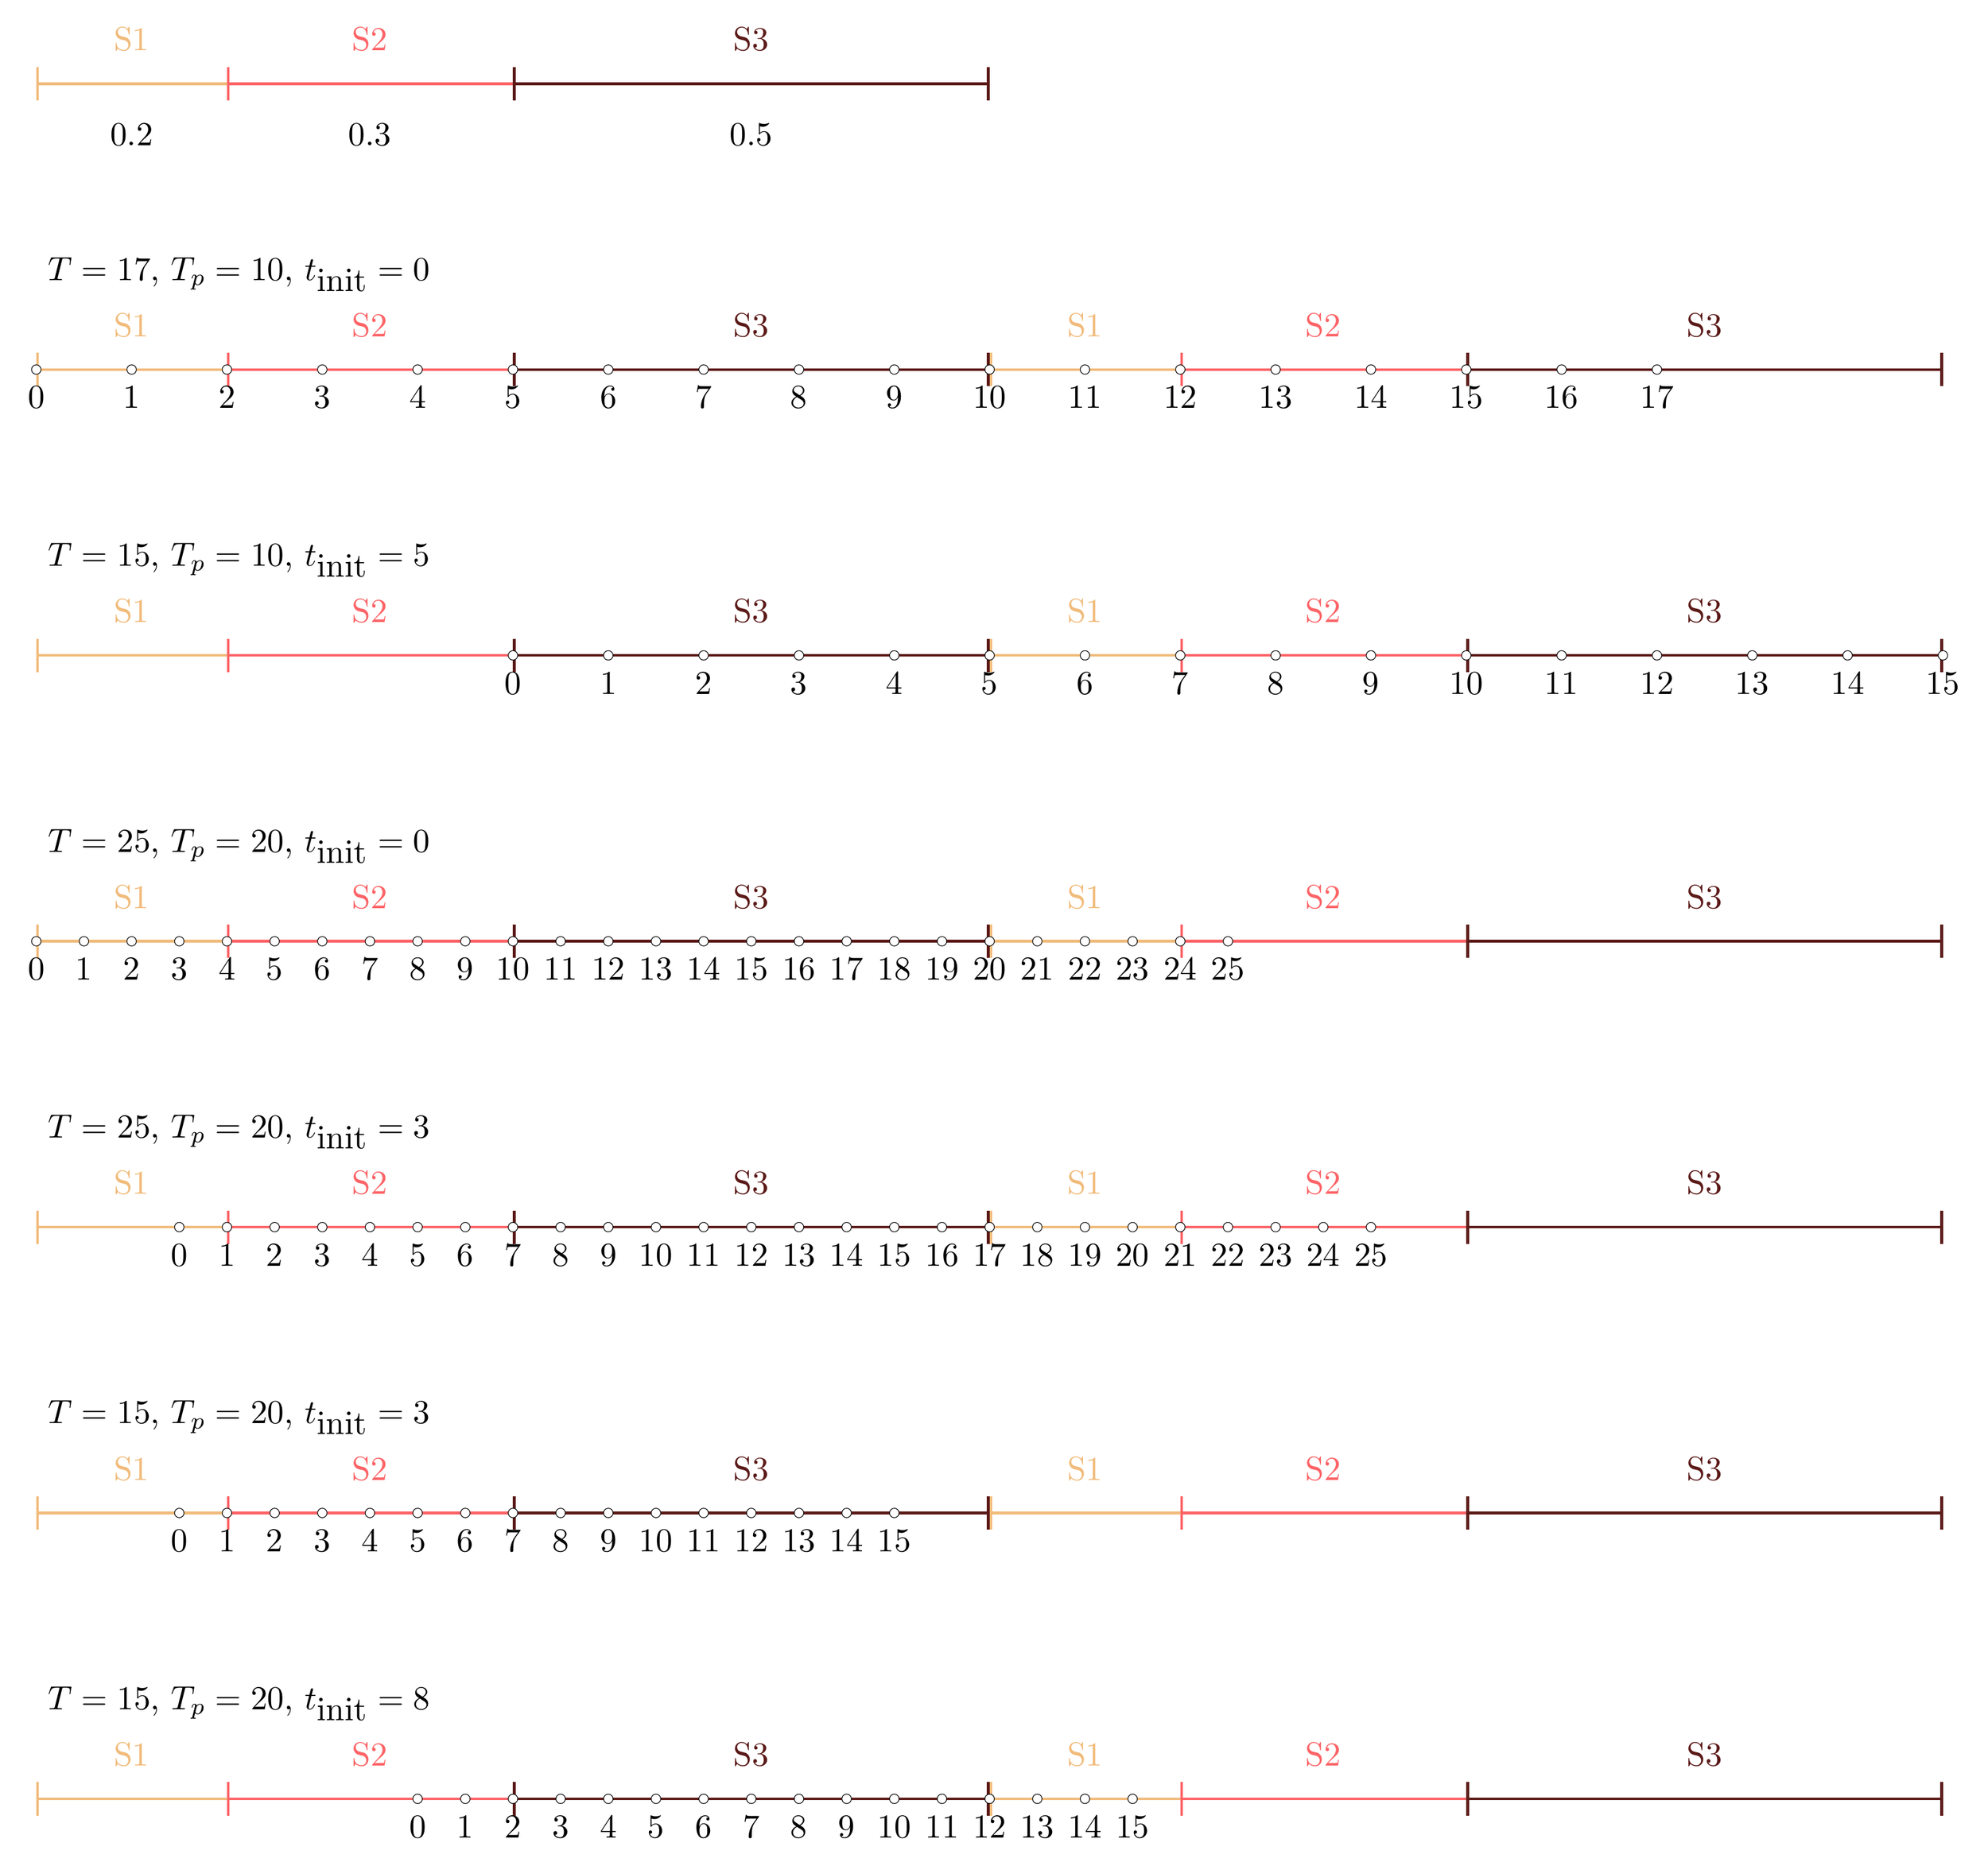
\begin{tikzpicture}
[scale=2,node distance=1cm, transform shape,
arr/.style={-{Latex[width=10mm]}},
tic/.style={circle,inner sep=1pt,draw,fill=white}]
%%%%%%%%%%
\def \period {10}
\newcommand{\ts}{t_{\textrm{init}}}

\newcommand{\seasons}[2]{
\begin{scope}[shift={(#1,#2)}]
    \path[ultra thick,s1,{|[width=7mm]}-] (0,0) edge[above] node (s1) [shift={(0,.2)}] {S1} (2,0);
    \path[ultra thick,s2,{|[width=7mm]}-] (2,0) edge[above] node (s2) [shift={(0,.2)}] {S2} (5,0);
\path[ultra thick,s3,{|[width=7mm]}-{|[width=7mm]}] (5,0) edge[above] node (s3) [shift={(0,.2)}] {S3} (\period,0);
\end{scope}
}
%%%%%%%%%%

\newcommand{\tics}[4]{
\def \y {#1}
\def \timesteps {#2}
\def \timestepsPerPeriod {#3}
\def \start {#4}
\begin{scope}[shift={(0,\y)}]
\node[anchor=west] {$T=\timesteps$, $T_p=\timestepsPerPeriod$, $\ts=\start$};
\seasons{0}{-1}
\seasons{10}{-1}
\foreach \a in {0,...,\timesteps}
\node[tic,label=below:$\a$] (a\a) at
({\period/\timestepsPerPeriod*\start+\period/\timestepsPerPeriod*\a},-1) {};
\end{scope}
}

%% setup
\begin{scope}[shift={(0,0)}]
\seasons{0}{0}
\node[below of=s1] {0.2};
\node[below of=s2] {0.3};
\node[below of=s3] {0.5};
\end{scope}

%% example 1
\tics{-2}{17}{10}{0}

%% example 2
\tics{-5}{15}{10}{5}

%% example 3
\tics{-8}{25}{20}{0}

%% example 4
\tics{-11}{25}{20}{3}

%% example 5
\tics{-14}{15}{20}{3}

%% example 5
\tics{-17}{15}{20}{8}
\end{tikzpicture}
\end{document}


